\chapter{Design}
Dette kapitel indeholder en beskrivelse af design valgene for Firebase databasen og applikationen, samt hvordan disse er implementeret. \\

\section{Firebase database} \label{sec:FirebaseDesign}
\chapter{Firebase}
Firebase\cite{Firebase} er en development platform til mobile applikationer, som Google står bag. Firebase tilbyder forskellige slags funktionaliter til både Android og iOS applikationer. Herunder beskrives disse produkter fra Firebase, som Ramboell App benytter sig af: \\

\textbf{Authentication\cite{FirebaseAuth}}
\begin{itemize}[-]
	\itemsep 0.3em 
	\item[] Firebase Authentication giver en række funktioner indenfor User Management, der gør det let at logge på, opret og log af. Firebase Authentication tilbyder en række forskellige muligheder for login fra mail eller en andet sociale medier, som Facebook, Twitter osv, til både Android og iOS applikationer, af disse vælger vi at benytte mail som login for. Bruger data som E-mail, navn og crypteret password, vil blive gemt i Firebase, og derfor vil der ikke være behov for, at Rambøll Danmark A/S skal sørge for at opsætte server med en bruger database, forbindelsen op til serveren og derefter vedligeholdelse. 
	
\end{itemize}	
\textbf{Realtime Database\cite{FirebaseRealtimeDB}}
\begin{itemize}[-]
	\itemsep 0.3em 
	\item[]  Firebase Realtime Database er et NoSQL cloud database, der gemmer data'en som JSON\cite{JSON}, med mulighed for synkroniser data med alle som benytter Ramboell App, der har forbindelse til internet. Databasen er Cloud hosted, hvilket betyder at som udviklere vil det give en "serverless" miljø at arbejde med, hvor arbejde med opsætning og vedligeholdelse af server vil ikke være nødvendigt. Et af de store fordele er at det er en realtime database, der synchroniser data automatisk. Når der modtages ændringer i data vil enhver device der er koblet til internet modtage notifikationen om ændringen, og kan begynde at hente det ned. 
\end{itemize}
\textbf{Firebase Storage}
\begin{itemize}[-]
	\itemsep 0.3em 
	\item[] Tilsvarende Firebase Database er Cloud Storage tilregnet for filer, som video, billeder eller andre tilsvarende data. I denne tilfælde bliver Firebase Storage benyttet til at gemme på PDF objecter som brugeren hente og uploade. Et vigtigt egenskab Storage har er at den er bygget til at genoptage download af filer i tilfælde af ustabilt internet. Hvilket kan være tilfældet hos Rambøll hvis de skal ud til konstruktions arbejde på et motorvej hvor forbindelse er ikke lige så optimalt som i byen. 
\end{itemize}

\textbf{Firebase}
I følgende afsnit redegøres for de beslutninger der tages angående valg af Firebase. \\
Firebase kræven næsten næsten ingen setup at bruge, hvilken var et af de store plus for hvorvidt hvilke teknologier der bruges iforhold til Ramboell App. 
For at starte Firebase i Android og iOS, skal man have en google account, og oprette en projekt i google. Derefter skal man blot add firebase til ens app, og tilføje de bibloteker man har behov for.
Det giver et let adgang til data, brugere og filer pågrund af de bibloteker der udstilles. 
Et andet grund til Firebase er at der er ikke behov for at sætte en server op, og fordi at Ramboell ikke lægger en server tilrådighed er dette til oplagt mulighed.

Et af ulemperne med firebase er deres pris der kan blive dyrt hvis applikationen bliver brugt meget, \cite{{FirebasePricing}}, men da det er kun beregnet som inhouse applikation med ca. 10 bruger er dette acceptablet.


\textbf{Database}\\
I følgende afsnit redegøres for de beslutninger der tages angående valg af database. SQL eller NoSQL.
Der er fordele og ulemper ved begge database typer herunder nævnes nogle af forskellige mellem disse to typer.

\textbf{database modellen} \\
Ved SQL database kræves der Schema, som definerer data modellen, og danner et billede af hvad og hvordan data skal struktureres, os kaldes et table. Ved NoSQL som er "schema-less", er det op til brugeren at definere en data model. NoSQL mere fleksibelt når det omhandler ændringer i data modellen, men ligger mere ansvar hos udvikleren at modellere dataen optimalt. Men ved valget af et andet database betyder dette, at der vil være et server applikation, opstilling af database og vedligeholdelse af det. 

\textbf{Queries}
Når data skal hentes tilbyder SQL database JOIN, hvor data fra flere tabler flettes sammen og returneres. Noget som man ikke har i NoSQL database. For at få tilsvarende effekt skal applikationen query flere gange og sammensætte resultatet selv.  

\textbf{Transactions}
SQL tilbyder transaction, hvis man skal have transaction tilsvarende effekt på NoSQL skal man selv sørge for det i applikations kode.
 
\textbf{Skalering}
Efterhånden som applikationen bliver brugt, vokser mængden af lagret data skal stillingen tages om man vel skalerer sin server op eller skalerer ud ved at tilføje et server. Problemmet ved at lave en større server er at der kommer et tidspunkt, hvor det vil blive for dyrt at købe en større server, hvor man vil hellere skalere ud. Fordelen ved NoSQL har over SQL database er at det er lettere at skalere ud, men
når man kigger på at det er en inhouse projekt til Ramboell vil der være begrænset antal brugere til systemet, og mængden af data der vokser vil være i begrænset omfang, og derfor er det ikke være noget reelt betydning for denne projekt. 


\section{Applikation} \label{sec:ApplikationDesign}
Implementeringen af applikationen sker i Xamarin iOS, da der i analysen var blevet overset nogle begrænsninger i forhold til funktionaliteten når der skulle arbejdes med PDF'er i Xamarin Forms\cite{Forms}. \\ \\
Til udvikling af applikationen er der brugt et MVC design \cite{MVC}, som vist herunder, på figur \ref{fig:MVC}
\begin{figure}[H] % (alternativt [H])
	\centering
	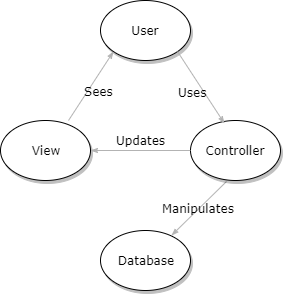
\includegraphics[height=8cm, width=8cm]{../ArkitekturDesign/Design/MVC}
	\caption{MVC design for Rambøll Tilsyn.}
	\label{fig:MVC}
\end{figure}

Model-View-Controller er et design pattern til opbygning af user interfaces. Model er der alt
data ligger. Det er så Controllerens opgave at manipulere det til Viewet. Viewet er det som
ses af brugeren og som der kan interageres med. Hvis brugeren interagerer med applikationen er
det Controllerns opgave at få det ned i Modellen og få kaldt det nye view frem. \\
Modellen i Rambøll Tilsyn, ligger i Firebase.
Der er brugt MVC design pattern til alle views i applikationen.

\clearpage

\subsection{Navigationstræ}
Figur \ref{fig:Navi} viser et navigationstræ for Rambøll Tilsyn. Her ses flowet gennem appliaktionen og hvordan man kan til gå de forskellige views.

\begin{figure}[H] % (alternativt [H])
	\centering
	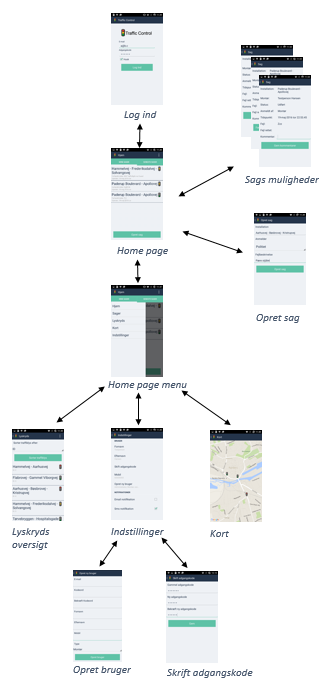
\includegraphics[height=20cm, width=12cm]{../ArkitekturDesign/Design/Navigation/Navigation}
	\caption{Navigations træ for Rambøll Tilsyn.}
	\label{fig:Navi}
\end{figure}

\clearpage
\section{Login}

\begin{figure}[H] % (alternativt [H])
	\centering
	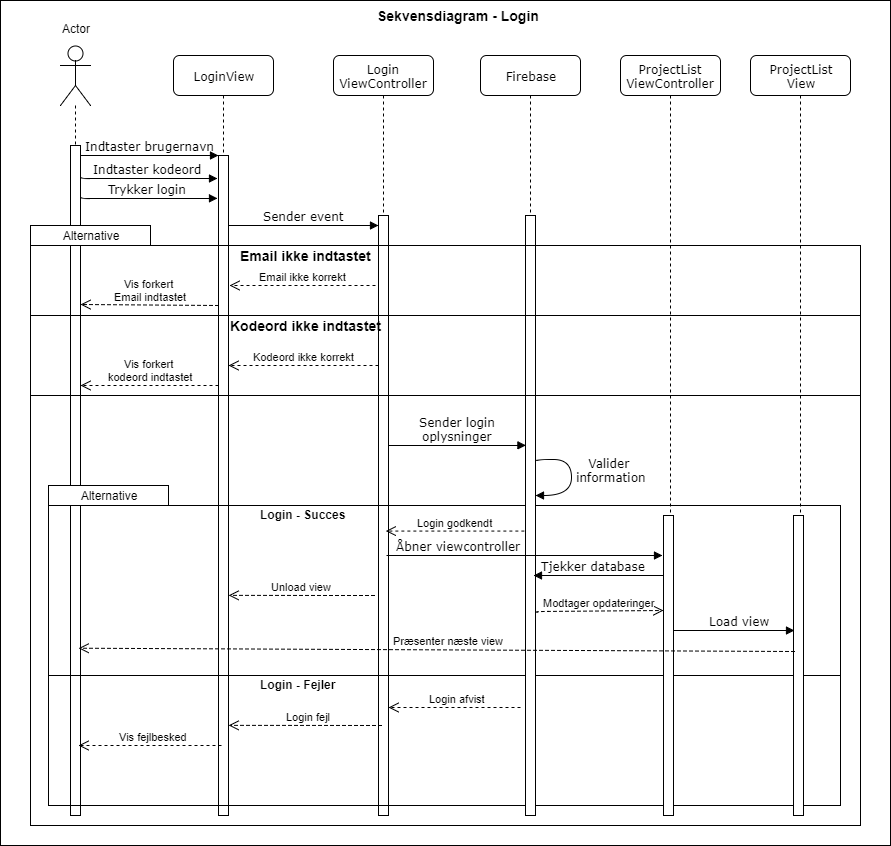
\includegraphics[width=1.1\textwidth]{../ArkitekturDesign/Design/Login/LoginSekvensDiagram}
	\caption{Sekvensdiagram for Login i Rambøll Tilsyn.}
	\label{fig:LoginSekvens}
\end{figure}
\subsection{Projekt Oversigt} \label{sec:ProjectList}
Dette afsnit indeholder en gennemgang af den grafisk brugergrænseflade, design og implementering af 'Project List' viewet i Rambøll Tilsyn.

\subsubsection{Design}
På Figur \ref{fig:ProjctListSekvens} ses sekvensdiagrammet for 'Project List' viewet til Rambøll Tilsyn.
\begin{figure}[H] % (alternativt [H])
	\centering
	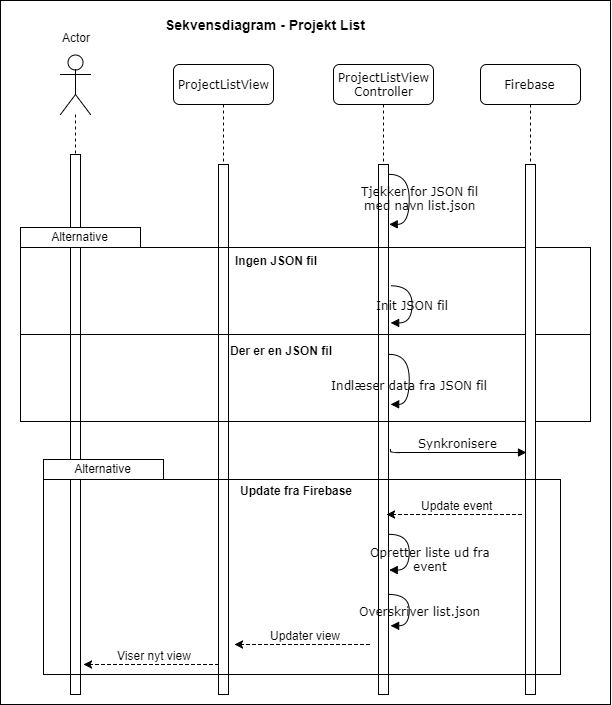
\includegraphics[height=15cm, width=15cm]{../ArkitekturDesign/Design/ProjectList/ProjektListSekvensDiagram}
	\caption{Sekvensdiagram for ProjectList i Rambøll Tilsyn.}
	\label{fig:ProjctListSekvens}
\end{figure}

\clearpage

\subsubsection{Grafisk brugergrænseflade}
I ProjectListViewet er der en oversigt over, hvilke projekter der ligger i databasen, samt mulighed for øverst at tilføje projekt eller tilføj bruger. Se Figur \ref{fig:ProjectListView}
\begin{figure}[H] % (alternativt [H])
	\centering
	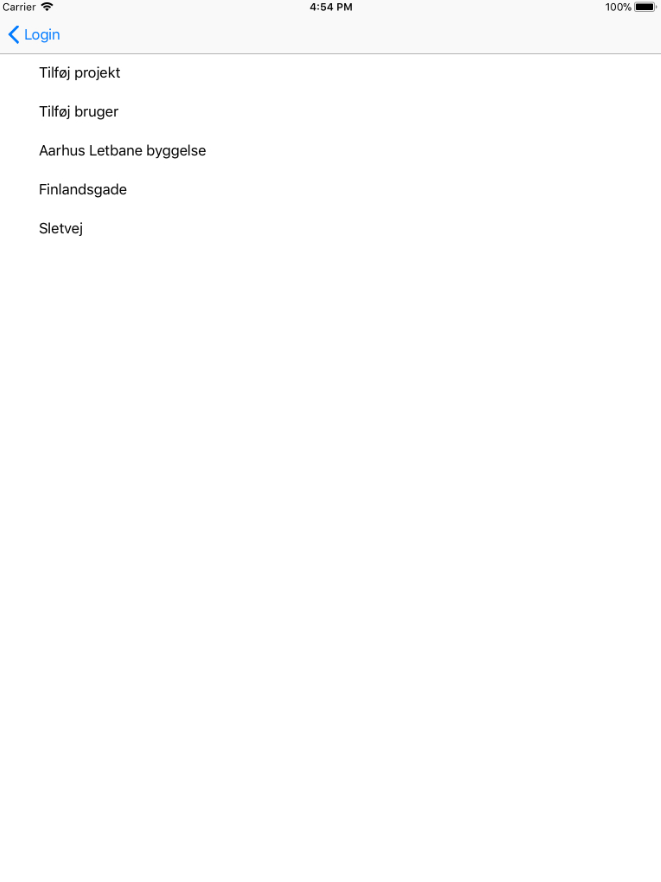
\includegraphics[height=12cm, width=10cm]{../ArkitekturDesign/Design/ProjectList/ProjectList}
	\caption{'Project List' viewet, som det er implementeret i Rambøll Tilsyn.}
	\label{fig:ProjectListView}
\end{figure}

\clearpage

\subsubsection{Implementering}
I dette afsnit vil der blive beskrevet funktionaliteten for de vigtigste funktioner i koden tilhørende 'Project List' viewet.

På Figur \ref{fig:ProjectListViewController}, ses funktionen for ProjectListViewController().
\begin{figure}[H] % (alternativt [H])
	\centering
	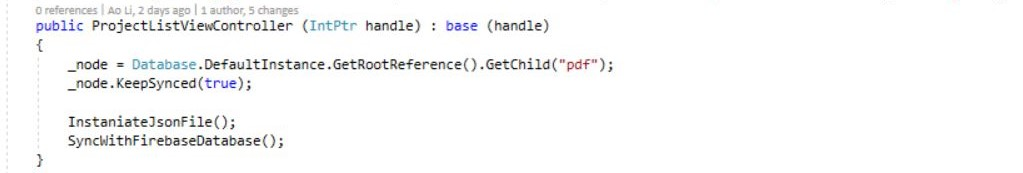
\includegraphics[height=3cm, width=17cm]{../ArkitekturDesign/Design/ProjectList/ProjectListViewController}
	\caption{Kode snip - ProjectListViewController() fra ProjectListViewController.cs}
	\label{fig:ProjectListViewController}
\end{figure}
Det første er, at der hentes en reference node med navn PDF fra Firebase og fortæller at denne node skal holdes synkroniseret, i tilfælde af dataændring. \\
Efterfølgende initialiseres JSON-filen og synkrorinisere efterfølgende med Firebase.

På Figur \ref{fig:JSONFile}, ses funktionen for InstaniateJsonFile().
\begin{figure}[H] % (alternativt [H])
	\centering
	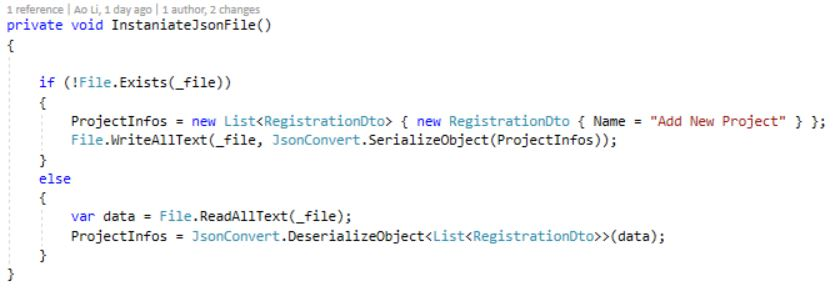
\includegraphics[height=5cm, width=15cm]{../ArkitekturDesign/Design/ProjectList/JSONFile}
	\caption{Kode snip - InstaniateJsonFile() fra ProjectListViewController.cs}
	\label{fig:JSONFile}
\end{figure}
Der oprettes en JSON-fil, hvis der ikke findes en i forvejen. Denne gemmes lokalt.\\
Hvis der findes en JSON-fil, læses data fra filen.

\clearpage

På Figur \ref{fig:SyncWithDB}, ses funktionen for SyncWithFirebaseDatabase().
\begin{figure}[H] % (alternativt [H])
	\centering
	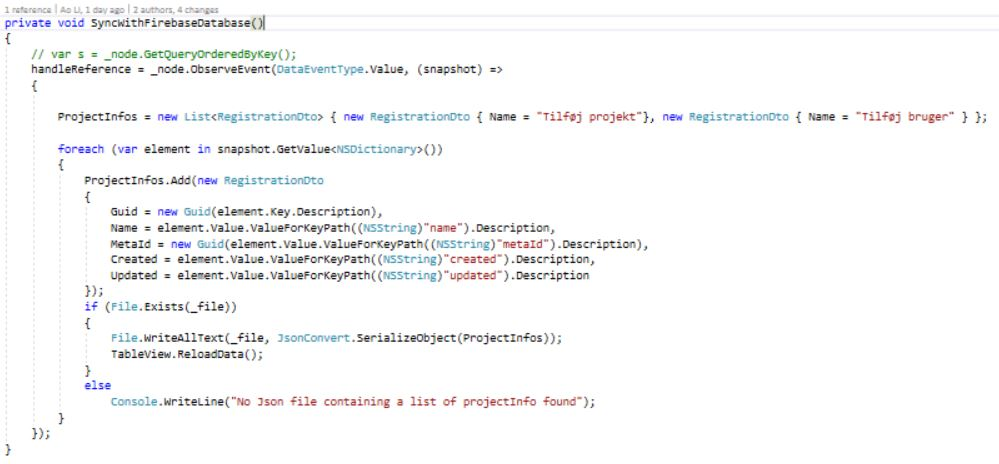
\includegraphics[height=8cm, width=15cm]{../ArkitekturDesign/Design/ProjectList/SyncWithDB}
	\caption{Kode snip - SyncWithFirebaseDatabase() fra ProjectListViewController.cs}
	\label{fig:SyncWithDB}
\end{figure}
Noden, som er oprettet i konstrukteren, som ses på Figur \ref{fig:ProjectListViewController}, den vedhæftes til et event, som kaldes hver gang noden ændres. \\
Når eventet kaldes, læses data fra eventet og gemmer dette i JSON filen. Efterfølgende fortælles controlleren at viewet skal opdateres.

På Figur \ref{fig:ViewDidLoad}, ses funktionen for ViewDidLoad().
\begin{figure}[H] % (alternativt [H])
	\centering
	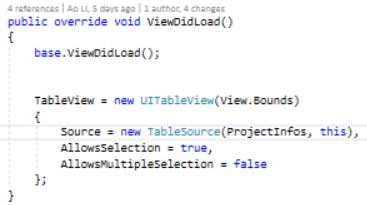
\includegraphics[height=5cm, width=10cm]{../ArkitekturDesign/Design/ProjectList/ViewDidLoad}
	\caption{Kode snip - ViewDidLoad() fra ProjectListViewController.cs}
	\label{fig:ViewDidLoad}
\end{figure}
Her sættes ListViewets source til at være TableSource.

\clearpage

På Figur \ref{fig:TableSource}, ses funktionen for TableSource().
\begin{figure}[H] % (alternativt [H])
	\centering
	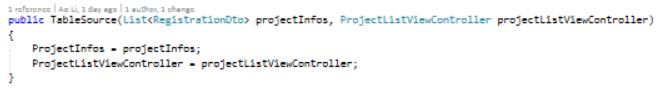
\includegraphics[height=2cm, width=15cm]{../ArkitekturDesign/Design/ProjectList/TableSource}
	\caption{Kode snip - TableSource() fra TableSource.cs}
	\label{fig:TableSource}
\end{figure}
Der initialiseres, hvilke værdier der skal fremvises og der er givet en reference til ProjctListViewControlleren.

På Figur \ref{fig:RowSelection}, ses funktionen for RowSelected().
\begin{figure}[H] % (alternativt [H])
	\centering
	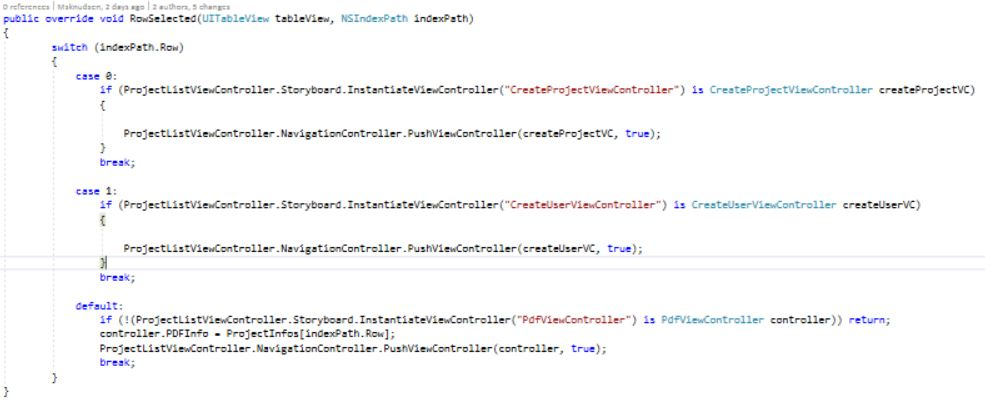
\includegraphics[height=8cm, width=17cm]{../ArkitekturDesign/Design/ProjectList/RowSelection}
	\caption{Kode snip - RowSelected() fra TableSource.cs}
	\label{fig:RowSelection}
\end{figure}
Der er en switch case, case CreateProject giver bruger mulighed for at navigere til 'Opret projekt' siden. Case CreateUser navigere brugeren til 'Opret bruger' siden. \\
Ellers skal den navigere brugeren til 'PDFViewControlleren', for det valgte projekt.

\clearpage

\section{Accepttest for Opret bruger (CRS-2)}
Dette afsnit beskriver accepttesten for Opret bruger.

\textbf{User story beskrivelse} \\
Som bruger \\
Ønsker jeg at kunne oprette en bruger på applikationen \\
For at kunne give en anden bruger adgang til systemet

\begin{table}[H]
	\centering
	\begin{tabular}{|ll|l|ll|} \hline
		\textbf{Scenarie} &  & \textbf{Beskrivelse}&  \textbf{Godkendt}&  \\ \hline
		Opret bruger&  &  Når alt information omkring en bruger &  OK&  \\
		& & er udfyldt, og der trykkes opret bruger, bliver brugeren oprettet& & \\ \hline
	\end{tabular}
	\caption{Accepttest for Opret bruger (CRS-2)}
	\label{AcceptOpretBruger}
\end{table}

\clearpage
\section{Accepttest for Opret projekt (CRS-16)}
Dette afsnit beskriver accepttesten for Opret projekt.

\textbf{User story beskrivelse} \\
Som bruger \\
Ønsker jeg at kunne oprette projektoplysninger \\
For at have aktuelle oplysninger om projektet

\begin{table}[H]
	\centering
	\begin{tabular}{|ll|l|ll|} \hline
		\textbf{Scenarie} &  & \textbf{Beskrivelse}&  \textbf{Godkendt}&  \\ \hline
		Opret projekt&  &  Når alt information omkring et projekt &  Ikke OK&  \\
		& & er udfyldt, og der trykkes opret projekt, bliver brugeren oprettet& & \\ \hline
	\end{tabular}
	\caption{Accepttest for Opret projekt (CRS-16)}
	\label{AcceptOpretProjekt}
\end{table}
\subsection{Registrering på PDF}

\subsubsection{Grafisk brugergrænseflade}

\subsubsection{Design \& Implementering}

\subsection{Eksportering} \label{sec:Login}
Dette afsnit indeholder en gennemgang af grafisk brugergrænseflade, design og implementering af 'Export viewet' i Rambøll Tilsyn.

\subsubsection{Design}
På figur \ref{fig:EksporterSekvensDiagram} ses sekvens diagrammet for 'Export' viewet til Rambøll Tilsyn.
\begin{figure}[H] % (alternativt [H])
	\centering
	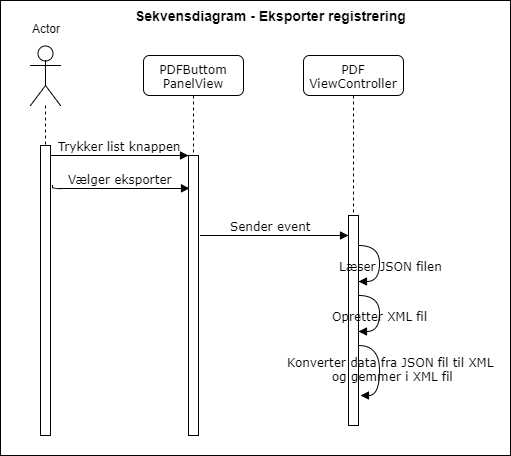
\includegraphics[height=10cm, width=10cm]{../ArkitekturDesign/Design/Eksportering/EksporterSekvensDiagram}
	\caption{Sekvensdiagram for Eksportering i Rambøll Tilsyn.}
	\label{fig:EksporterSekvensDiagram}
\end{figure}

\clearpage

\subsubsection{Grafisk brugergrænseflade}
Efter at have eksporteret registreringen til en XML fil, vil den se ud som på figur \ref{fig:Excel}.
\begin{figure}[H] % (alternativt [H])
	\centering
	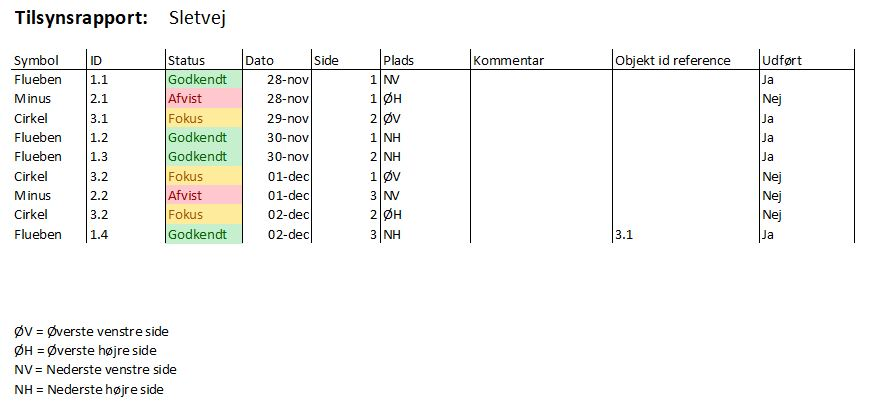
\includegraphics[height=10cm, width=17cm]{../ArkitekturDesign/Design/Eksportering/Excel}
	\caption{Export viewet som det vil se ud når det er åbent i excel.}
	\label{fig:Excel}
\end{figure}
Tabellen består af linjer hvor at hvert objekt har følgende information: \\
\textbf{Symbol:} Er navnet på den type symbol som er oprettet. \\
\textbf{ID:} Er objektets id. Dette gives ud fra hvilken type symbol det er. \\
\textbf{Status:} Viser statussen på objektet. Status følger typen af objekt. \\
\textbf{Dato:} Viser datoen for hvornår objektet er oprettet. \\
\textbf{Side:} Viser hvilken side i PDF tegningen objektet er oprettet på. \\
\textbf{Plads:} Viser hvor på den tilhørende side at objektet er placeret. \\
\textbf{Kommentar:} Giver mulighed for at uddybe eventuelle kommentar til objektet. \\
\textbf{Objekt id reference:} Hvis et objekt bliver ændret fra f.eks. et minus til et flueben, vil der blive oprettet et nyt fluebens objekt, som så får reference id til det minus, som er ændret til. \\
\textbf{Udført:} Viser om objektet er blevet udført. F.eks. at alle minus og cirkel objekter er blevet ænderet et flueben. \\

\subsubsection{Implementering}

\clearpage